\chapter{Report}

The goal is to make a sequencer. This sequencer takes footage from a camera mounted to a (racing) car and based on this it should be able to estimate the path the car has travelled. This process can be divided in multiple parts. The first part is to make a simple sequencer that can handle a stream of images and display them. The footage from the camera is a video, to process this, each frame of the video is stored as a separate image. These images can be fed to the sequencer to display them. The sequencer stores a predefined amount of images in a buffer and displays the first image in the buffer. With specific keys, it is possible to go forwards and backwards through the sequence. When advancing through the sequence, the next image is displayed and a new image is loaded in the buffer, erasing the previous image. Going backwards through the buffer is analogous. It's also possible to jump multiple frames ahead/backwards. The buffer is then cleared and filled with the correct images. For now, the images are loaded in grayscale. The big advantage is that a grayscale image only has one third of the information of an image in color with the same dimensions. Computationally everything will be faster using grayscale instead of color images. The drawback is a loss of information, but that drawback is rather small. The color of the image doesn't give us much more information to recognise structure and detect keypoints. So it's not worth the extra computations. However, in the footage we're using, the road is marked by colored cones. Most of the time the road is marked by yellow cones but sometimes there are blue cones on the road which means the car should slalom in between these cones. If at one point it should turn out the color of the cones is necessary, this won't be a problem. The original color image is always kept, if we want to determine the color of the cone, this can easily be done by looking at the area where the cone is on the original image.

The next step is preprocessing the images, preparing them for the actual processing. As said before, the images are loaded as grayscale images. Next to that, the images are getting cropped. We're only interested in what is going on below the horizon, everything above it won't give us much information so the. Right now, there isn't much to be cropped, because the footage we have is from a camera that was mounted tilted. Now that the sky and everything above the horizon is cropped out, there is one part of preprocessing left. The car itself is not moving relative to the camera, as the camera is fixed to the car, so it's irrelevant for the estimation of the movement. A mask is created to erase the car from the footage. This is only done when displaying the image however, otherwise the computation of keypoints wouldn't go well. When detecting the keypoints in the next step, keypoints laying in the area masked out by the ego-car, can be removed as keypoints. Figure \autoref{fig:input_image} shows an example of a frame before it is preprocessed. Figure \autoref{fig:output_image} shows the image after preprocessing. The black part is the ego-car.

\begin{figure}
    \centering
    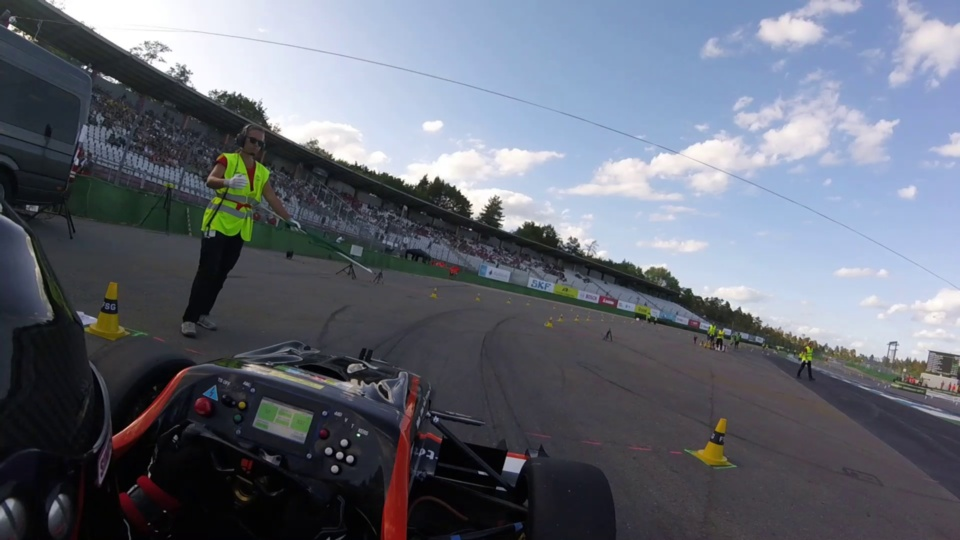
\includegraphics[width=1\textwidth]{figures/input_image.jpg}
    \caption{Input image}
    \label{fig:input_image}
\end{figure}

\begin{figure}
    \centering
    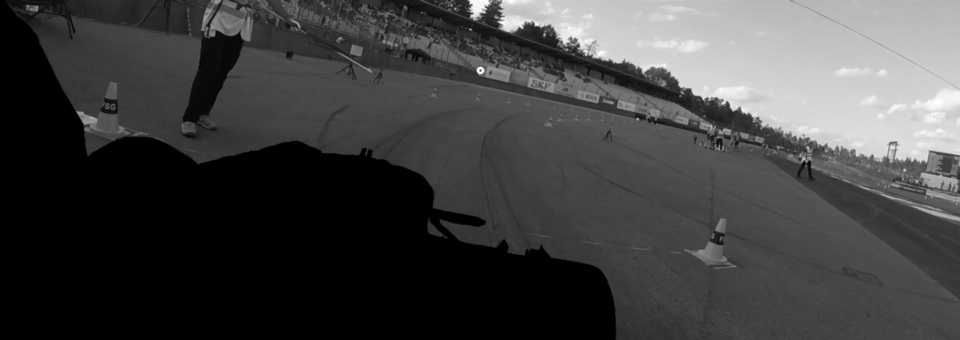
\includegraphics[width=1\textwidth]{figures/output_image.jpg}
    \caption{Preprocessed image}
    \label{fig:output_image}
\end{figure}